\documentclass[8pt]{beamer}
\usetheme{Copenhagen}
\usecolortheme{beaver}

\setbeamertemplate{navigation symbols}{}
\setbeamertemplate{headline}{}
\setbeamercovered{transparent=.5}

\usepackage{graphicx}
\usepackage{listings}
\usepackage{xcolor}

% General document information
\author{
    \textbf{Student: Sepehr Mousavi} \\
    Teacher: Pablo Antolin Sanches
}
\title[Parallelization of the N-Body problem]{Parallel and GPU-accelerated algorithms for the N-body problem}
\subtitle[P-HPC]{MATH-454 Parallel and High-Performance Computing}
\institute[EPFL]{{École Polytechnique Fédérale de Lausanne}}
\date{\today}

\begin{document}

\frame{\titlepage}

\begin{frame}{Strong scaling of the parallel Barnes-Hut method}

    \begin{figure}
        \centering
        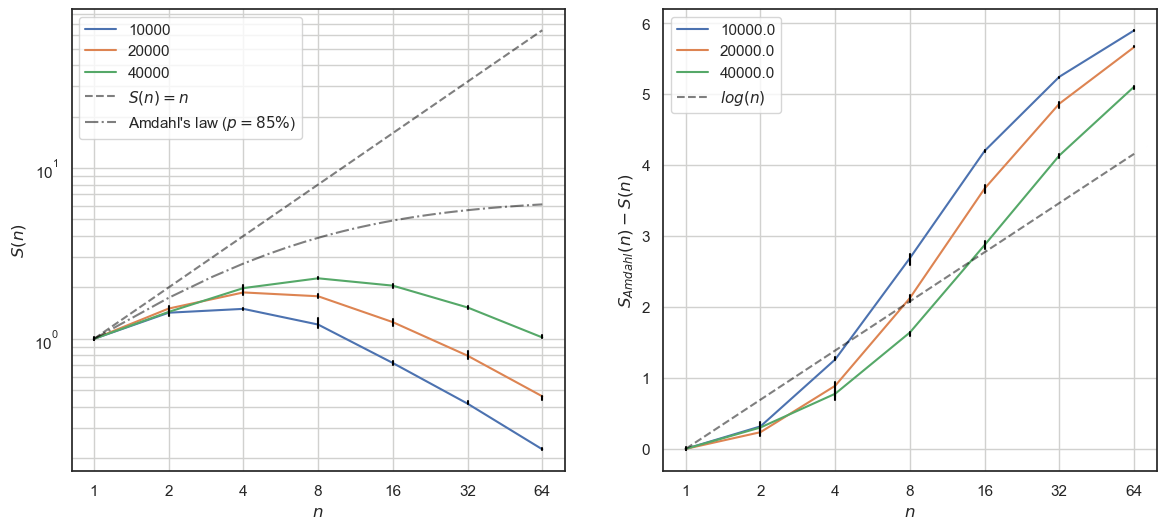
\includegraphics[width=.8\textwidth]{img/strongscaling.png}
    \end{figure}

  \begin{itemize}
    \item ...
    \item ...
  \end{itemize}

\end{frame}

\begin{frame}{Weak scaling of the parallel Barnes-Hut method}

    \begin{figure}
        \centering
        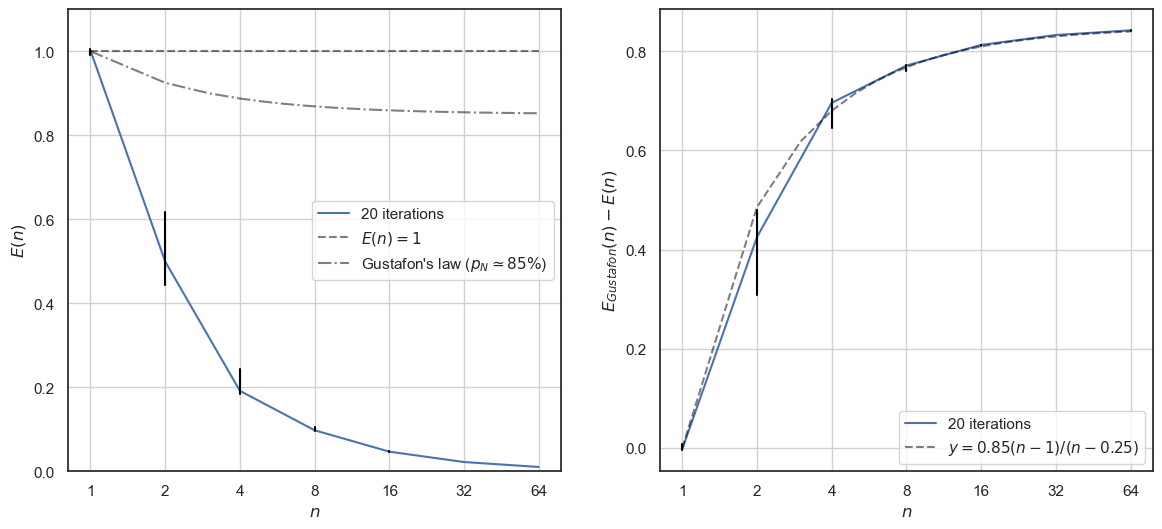
\includegraphics[width=.8\textwidth]{img/weakscaling.png}
    \end{figure}

    \begin{itemize}
    \item ...
    \item ...
    \end{itemize}

\end{frame}

\begin{frame}{Block sizes of the GPU-accelerated particle-particle method}

    \begin{columns}
        \column{.5\textwidth} {
            \centering
        }
        \column{.4\textwidth} {
            \centering
            \begin{figure}
                \centering
                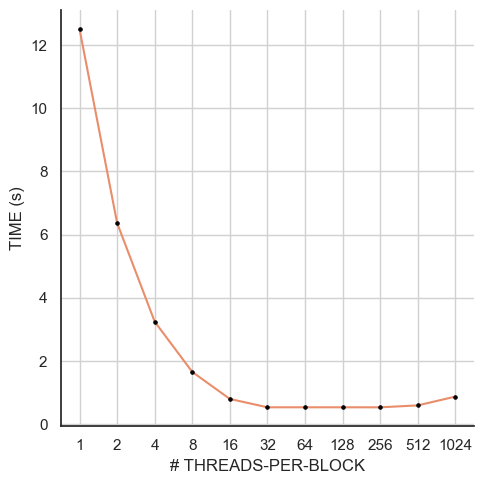
\includegraphics[width=\textwidth]{img/threadsperblock.png}
            \end{figure}
        }
    \end{columns}


\end{frame}



% \begin{frame}{Remarks and Prospect}

%     \textbf{Fixed dimensions:}
%     \begin{itemize}
%         \item The codes can be used as a static library.
%         \item Since the input and output dimensions are templated, the compiled executable is always limited to a set of pre-defined dimensions.
%         \item This behaviour can be changed by implementing dynamic memory allocation for \texttt{Vector}, \texttt{Function}, and \texttt{Workflow}.
%     \end{itemize}

%     \vfill

%     \textbf{Data types and memory allocation:}
%     \begin{itemize}
%         \item The data type of \texttt{Vector} (currently \texttt{double}) should be templated.
%         \item Since the size of the vectors (e.g., \texttt{n\_samples}) are always fixed, the code can benefit from static arrays (\texttt{std::array}) instead of vectors (\texttt{std::vector}).
%     \end{itemize}

%     \vfill

%     \textbf{Next steps:}
%     \begin{itemize}
%         \item The configurations of the source distribution can be loaded from an input file, similar to \texttt{Function}.
%         \item Histograms of the generated samples and convergence plots for the Central Limit Theorem can be added to the outputs.
%     \end{itemize}


% \end{frame}

\end{document}